% Name: Layered architecture
% Description: Four layers stacked from the user interface down to the database, each calling only the layer beneath it, with logging and security cutting across them all.
% Tags: layered architecture, n-tier, software architecture, separation of concerns

\usetikzlibrary{arrows.meta, shapes.geometric}

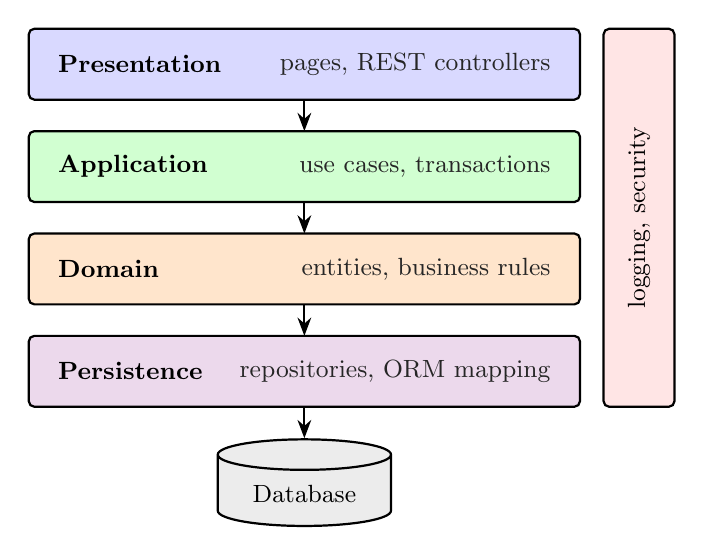
\begin{tikzpicture}[every node/.style={font=\small}, >={Stealth}]
  \foreach \i/\name/\what/\c in {0/Presentation/{pages, REST controllers}/blue!15, 1/Application/{use cases, transactions}/green!18, 2/Domain/{entities, business rules}/orange!20, 3/Persistence/{repositories, ORM mapping}/violet!15} {
    \draw[thick, fill=\c, rounded corners=2pt] (0,-1.3*\i) rectangle ++(7,-0.9);
    \node[anchor=west, font=\small\bfseries] at (0.25,-1.3*\i-0.45) {\name};
    \node[anchor=east, gray!30!black] at (6.75,-1.3*\i-0.45) {\what};
  }
  \foreach \i in {0,1,2} \draw[->, thick] (3.5,-1.3*\i-0.9) -- ++(0,-0.4);
  \draw[->, thick] (3.5,-4.8) -- ++(0,-0.4);
  \node[draw, thick, cylinder, shape border rotate=90, aspect=0.25, fill=gray!15, minimum width=22mm, minimum height=11mm, anchor=north] at (3.5,-5.2) {Database};
  \draw[thick, fill=red!10, rounded corners=2pt] (7.3,0) rectangle (8.2,-4.8);
  \node[rotate=90] at (7.75,-2.4) {logging, security};
\end{tikzpicture}
